\documentclass[a4paper,11pt]{article}
\usepackage{amssymb, enumitem}

\parindent 0cm
\usepackage{amssymb,amsmath,amsthm,latexsym,epsfig,euscript,multicol}
\usepackage[utf8x]{inputenc}
\usepackage{listings,xcolor,bm}


\definecolor{mygreen}{rgb}{0,0.6,0}
\definecolor{mygray}{rgb}{0.5,0.5,0.5}
\definecolor{mymauve}{rgb}{0.58,0,0.82}
\lstset{
  backgroundcolor=\color{white},   % choose the background color; you must add
  basicstyle=\small\ttfamily,      % the size of the fonts that are used for the code
  breakatwhitespace=false,         % sets if automatic breaks should only happen at whitespace
  breaklines=true,                 % sets automatic line breaking
  captionpos=b,                    % sets the caption-position to bottom
  commentstyle=\color{mygreen},    % comment style
  deletekeywords={...},            % if you want to delete keywords from the given language
  escapeinside={\%*}{*)},          % if you want to add LaTeX within your code
  extendedchars=true,              % lets you use non-ASCII characters; for 8-bits encodings only, does not work with UTF-8
  firstnumber=1,                % start line enumeration with line 1000
  frame=single,	                   % adds a frame around the code
  keepspaces=true,                 % keeps spaces in text, useful for keeping indentation of code (possibly needs columns=flexible)
  keywordstyle=\color{blue},       % keyword style
  language=Python,                 % the language of the code
  morekeywords={*,...},            % if you want to add more keywords to the set
  numbers=left,                    % where to put the line-numbers; possible values are (none, left, right)
  numbersep=5pt,                   % how far the line-numbers are from the code
  numberstyle=\tiny\color{mygray}, % the style that is used for the line-numbers
  rulecolor=\color{black},         % if not set, the frame-color may be changed on line-breaks within not-black text (e.g. comments (green here))
  showspaces=false,                % show spaces everywhere adding particular underscores; it overrides 'showstringspaces'
  showstringspaces=false,          % underline spaces within strings only
  showtabs=false,                  % show tabs within strings adding particular underscores
  stepnumber=5,                    % the step between two line-numbers. If it's 1, each line will be numbered
  stringstyle=\color{mymauve},     % string literal style
  tabsize=4,	                   % sets default tabsize to 2 spaces
  title=\lstname                   % show the filename of files included with \lstinputlisting; also try caption instead of title
}
% Caracteres especiales
\def\A{\mathbb{A}}
\def\C{\mathbb{C}}
\def \N{\mathbb{N}}
\def \P{\mathbb{P}}
\def \Q{\mathbb{Q}}
\def \R{\mathbb{R}}
\def \Z{\mathbb{Z}}
\def \sen{\textrm{sen}}

\def\Np{$\N$}
\def\Zp{$\Z$}
\def\Qp{$\Q$}
\def\Rp{$\R$}
\def\Cp{$\C$}

\def\bb{\bm{b}}
\def\bu{\bm{u}}
\def\bv{\bm{v}}
\def\bx{\bm{x}}
\def\bA{\bm{A}}
\def\bB{\bm{B}}
\def\bD{\bm{D}}
\def\bE{\bm{E}}
\def\bM{\bm{M}}
\def\bT{\bm{T}}


\def\K{\textrm{K}}
\def\V{\textrm{V}}
\def\S{\textrm{S}}

\def\degres{$^\circ$}

\newcount\todno
\def\no{\global\advance\todno by 1 \the\todno}

\topmargin-2cm \vsize 29.5cm \hsize 21cm
\setlength{\textwidth}{16.75cm}\setlength{\textheight}{23.5cm}
\setlength{\oddsidemargin}{0.0cm}
\setlength{\evensidemargin}{0.0cm}


\theoremstyle{definition}
\newtheorem{ejer}{Ejercicio}
\newcommand{\bej}{\begin{ejer}}
\newcommand{\fej}{\end{ejer}}

\begin{document}

\centerline{{\small Universidad de Buenos Aires - Facultad de Ciencias Exactas y Naturales - Ciencias de Datos}}

\vskip 0.2cm

\hrule

\vskip 0.2cm

 \centerline{{\bf\Large{\sc Laboratorio de Datos}}}

 \vskip 0.2cm

 \centerline{\ttfamily Primer Cuatrimestre 2024}

\vskip 0.2cm

 \hrule

 \bigskip
 \centerline{\bf Práctica N$^\circ$ 3: Visualizaci\'on de datos.}
 \bigskip


% \textbf{\large Visualizaci\'on}

\begin{enumerate}[resume]
\item Ten\'es datos de una encuesta realizada en distintas provincias de Argentina y quer\'es saber cu\'antas personas respondieron a la encuesta en cada provincia. ?`Hac\'es un gr\'afico de l\'ineas, de dispersi\'on (scatter), histograma o un gr\'afico de barras (bar plot)? Hac\'e a mano en tu cuaderno c\'omo esper\'as que se vea el gr\'afico.

\item Est\'as estudiando la relaci\'on entre altura y peso de las personas. Ten\'es un data-set que tiene como variables la edad, sexo y peso de cada persona. Si quer\'es describir estas variables por separado, ?`qu\'e gr\'afico har\'ias para cada una? ?`y si quer\'es visualizar la relaci\'on entre peso y altura? Hac\'e a mano en tu cuaderno c\'omo esper\'as que se vea el gr\'afico.

\item Hac\'e un gr\'afico de barras que muestre la cantidad de pa\'ises hay en cada continente seg\'un los datos de gapminder (recordar el ejercicio 1.4)

\item Quer\'es investigar c\'omo var\'ia la expectativa de vida entre los continentes. Para eso necesit\'as un gr\'afico como el siguiente:

\begin{center}
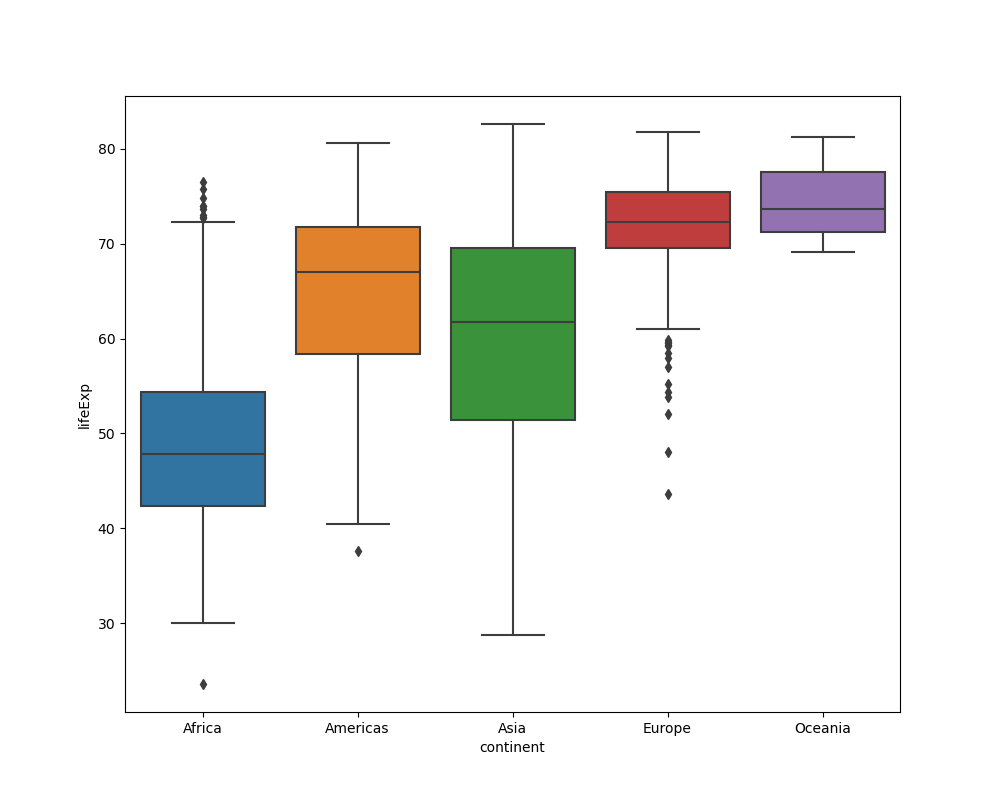
\includegraphics[scale=0.3]{practica3-img-gapminder-boxplot.png}
\end{center}

Reproduc\'i el gr\'afico de arriba reemplazando adecuadamente lo que falta en el siguiente c\'odigo:
\begin{lstlisting}
sns.boxplot(gapminder, x=COMPLETAR, y=COMPLETAR, order=sorted(COMPLETAR))
\end{lstlisting}

\item Reproducir el siguiente gr\'afico:

\begin{center}
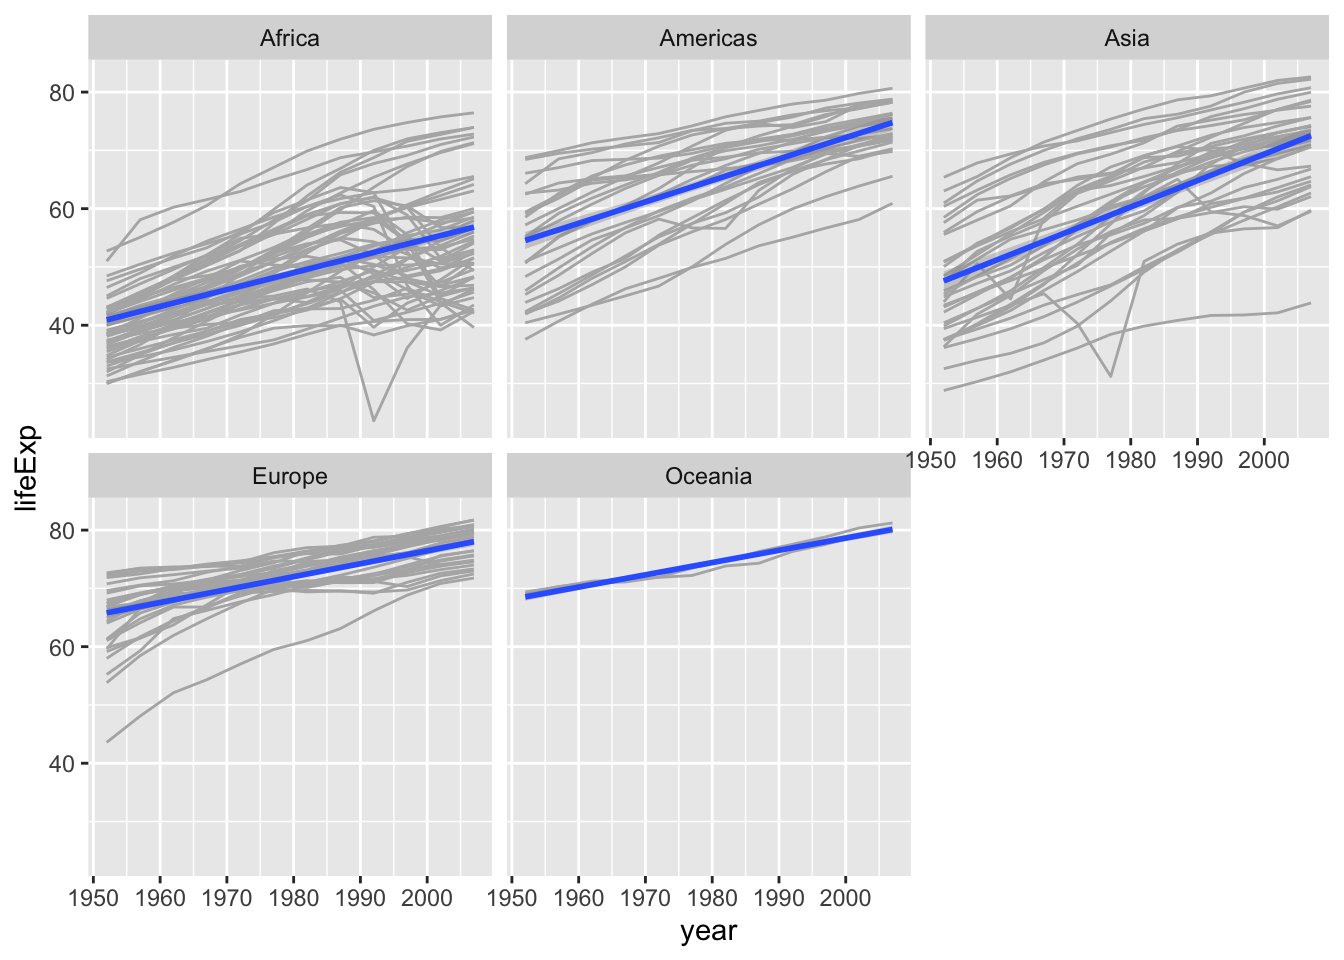
\includegraphics[scale=0.3]{practica3-img-gapminder-lifeExp.png}
\end{center}

\item (De ac\'a en adelante, trabajar con el dataset \lstinline{penguins} del paquete \lstinline{palmerpenguins}).
?`Cu\'antas
filas y
columnas hay en el dataset penguins?

\item  Dar una estad\'istica descriptiva de la variable \lstinline{bill_depth_mm}.

\item Hacer un \lstinline{scatterplot} de \lstinline{bill_depth_mm} (en el eje $y$) vs. \lstinline{bill_length_mm} (en el eje $x$).

\item ?`Cu\'al ser\'ia un buen geom para ver la relaci\'on entre \lstinline{species} y \lstinline{bill_depth_mm}?

\item Corregir el siguiente c\'odigo:
\begin{lstlisting}
ggplot(data = penguins) +
  geom_point()
\end{lstlisting}

\item ?`Qu\'e significa el argumento \lstinline{na.rm} en \lstinline{geom_point()}? Usando el dataset de \lstinline{palmerpenguins} crear un gr\'afico donde se requiera usar ese argumento como \lstinline{TRUE}.

\item Agregar un ``caption'' al gr\'afico de arriba. Ayuda: Mirar la documentaci\'on de \lstinline{labs()}.

\item Recrear la siguiente visualizaci\'on. ?`A qu\'e aes deber\'ia mapearse \lstinline{bill_depth_mm}? ?`El mapeo debe ser global o local?
\begin{center}
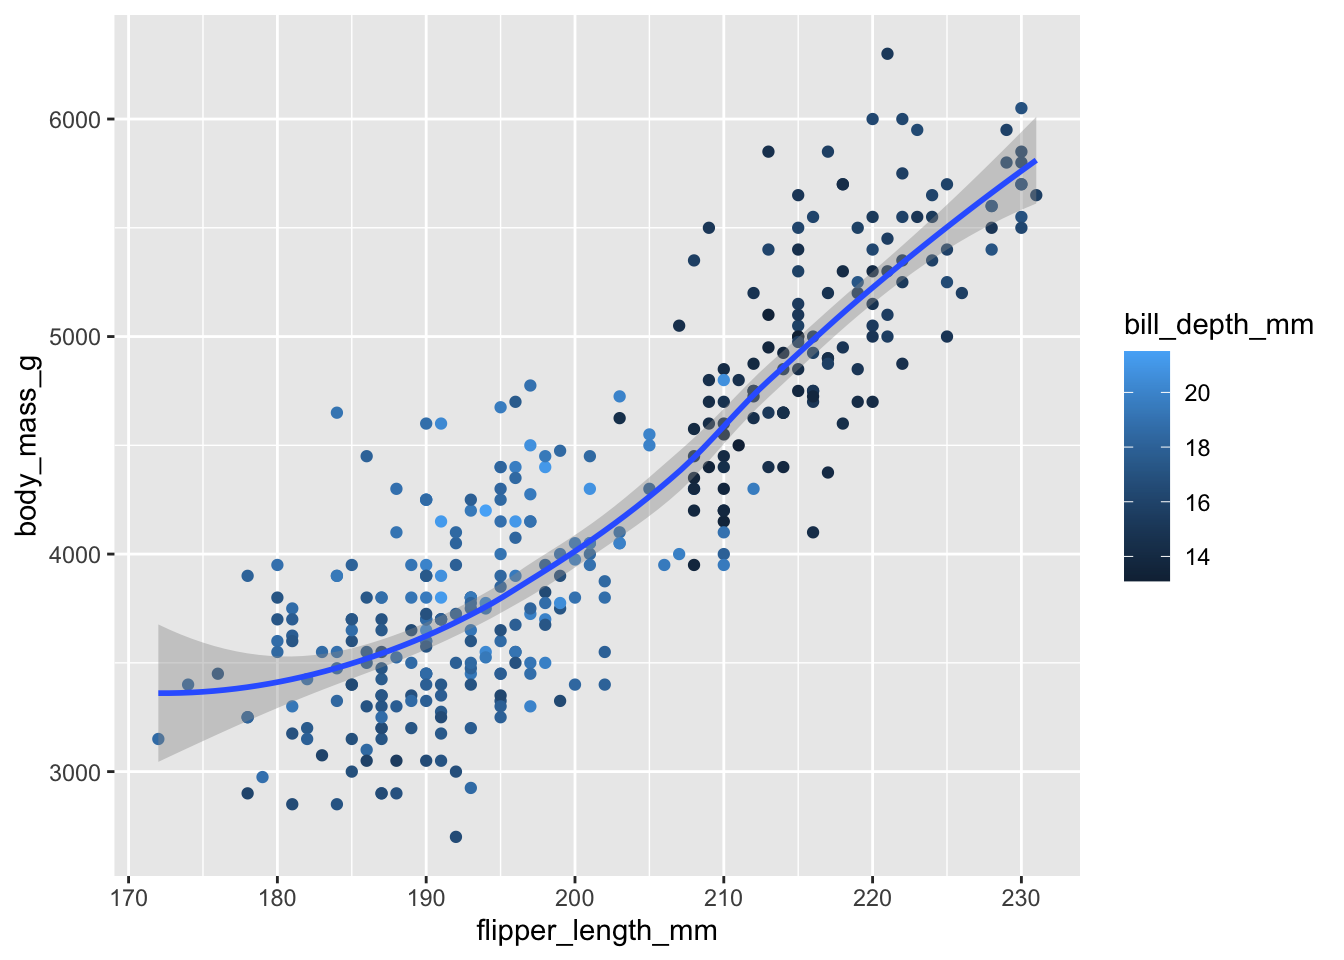
\includegraphics[scale=0.3]{practica3-img-penguins-mass.png}
\end{center}

\item Sin correr el c\'odigo, predecir qu\'e gr\'afico produce.
\begin{lstlisting}
ggplot(data = penguins,
       mapping = aes(x = flipper_length_mm, y = body_mass_g, color = island) ) +
  geom_point() +
  geom_smooth(se = FALSE)
\end{lstlisting}

\item Sin correr el c\'odigo, ?`estos dos gr\'aficos van a ser iguales o diferentes? ?`Por qu\'e?
\begin{lstlisting}
# grafico 1
ggplot(
  data = penguins,
  mapping = aes(x = flipper_length_mm, y = body_mass_g)
) +
  geom_point() +
  geom_smooth()

# grafico 2
ggplot() +
  geom_point(
    data = penguins,
    mapping = aes(x = flipper_length_mm, y = body_mass_g)
  ) +
  geom_smooth(
    data = penguins,
    mapping = aes(x = flipper_length_mm, y = body_mass_g)
  )
\end{lstlisting}

\item Sin correr el c\'odigo, predecir qu\'e gr\'afico produce.
\begin{lstlisting}
ggplot(data = penguins,
       mapping = aes(x = flipper_length_mm, y = body_mass_g, color = island) ) +
  geom_point() +
  geom_smooth(se = FALSE)
\end{lstlisting}

\item Sin correr el c\'odigo, ?`estos dos gr\'aficos van a ser iguales o diferentes? ?`Por qu\'e?
\begin{lstlisting}
# grafico 1
ggplot(
  data = penguins,
  mapping = aes(x = flipper_length_mm, y = body_mass_g)
) +
  geom_point() +
  geom_smooth()

# grafico 2
ggplot() +
  geom_point(
    data = penguins,
    mapping = aes(x = flipper_length_mm, y = body_mass_g)
  ) +
  geom_smooth(
    data = penguins,
    mapping = aes(x = flipper_length_mm, y = body_mass_g)
  )
\end{lstlisting}

\end{enumerate}

\end{document}


FACTORES


%%\item Las variables de clase "factor" (factores, o fct) son una clase especial que tiene R para trabajar con variables categ\'oricas. Una vez que se crean, los factores s\'olo pueden contener un conjunto pre-definido de valores que se conocen como los niveles del factor. ?`Qu\'e variables del dataset de gapminder son factores?
%
%\item Redefinir niveles. Supongamos que queremos cambiar la denominaci\'on del continente de Argentina a ``America'' (sin la s final). Prueben lo siguiente. ?`Qu\'e pas\'o? ?`Por qu\'e no funciona?
%\begin{lstlisting}
%class(gm.sur$continent)
%gm.sur$continent <- "America"
%class(gm.sur$continent)
%\end{lstlisting}
%
%Ahora prueben esto. ?`Entienden por qu\'e funciona?
%
%levels(gm.sur$continent) <- c("Africa", "America", "Asia", "Europe", "Oceania")
%class(gm.sur$continent)
%head(gm.sur)
%
%\item  Vamos a usar mucho "factores" a lo largo del curso, pero para que se den una idea, por ejemplo, los factores son muy \'utiles para codificar variables categ\'oricas en gr\'aficos. Vamos a ver esto bastante a lo largo de las clases, pero para que vean una aplicaci\'on simple, corran estas l\'ineas usando el paquete (que vamos a ver en las pr\'oximas clases) ggplot2.
%
%library(ggplot2)
%
%ggplot(data = gm.sur,
%       mapping = aes(x = year, y = pop, col = country)) +
%  geom_point(size = 3) +
%  theme_classic()
%
%Ahora corran lo siguiente. ?`En qu\'e difiere del anterior? ?`Pueden intuir por qu\'e tenemos ese resultado?
%
%ggplot(data = gm.sur,
%       mapping = aes(x = year, y = pop, size = country)) +
%  geom_point() +
%  theme_classic()
%
%?`Y si reemplazan size por shape dentro de aes(...)?
%
%4.13. Cambien m\'as cosas del c\'odigo anterior y prueben el resultado. De hecho, cambiar cosas y ver qu\'e pasa es una gran forma de aprender.

